\documentclass[tikz, margin=0.25mm]{standalone}

\begin{document}

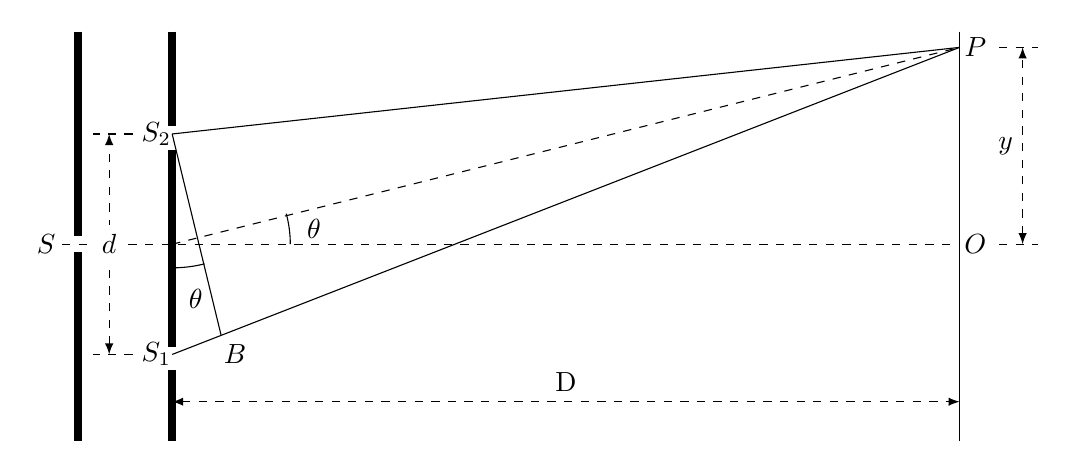
\begin{tikzpicture}[scale=0.1]  
\node [] () at (-2,49) {$S_2$}; 
\node [] () at (-2,21) {$S_1$}; 
\node [] (O) at (102,60) {$P$}; 
\node [] (M) at (102,35) {$O$}; 
\node [] () at (8,21) {$B$}; 
\draw [line width=0.1cm] (0,62) -- (0,50); 
\draw [line width=0.1cm] (0,47) -- (0,22); 
\draw [line width=0.1cm] (0,19) -- (0,10); 
\draw [line width=0.1cm] (-12,62) -- ++(0,-26);
\draw [line width=0.1cm] (-12,34) -- ++(0,-24);
\draw [] (100,62) -- (100,10); 
\draw [] (0,49) -- (100,60); 
\draw [] (0,21) -- (100,60); 
\draw (15,35) arc (0:15:15); 
\node at (18,37) {$\theta$}; 
\draw (0,32) arc (-90:-76:17); 
\node at (3,28) {$\theta$}; 
\draw [dashed] (0,35) -- (100,60); 
\draw [dashed] (-14,35) -- (100,35); 
\node [] (S) at (-16,35) {$S$};
\draw [dashed] (-5,49) -- (-10,49); 
\draw [dashed] (-5,21) -- (-10,21); 
\draw [dashed,<->,>=latex] (-8,21) -- (-8,49) node [fill=white,midway] {$d$}; 
\draw [dashed] (105,60) -- ++(5,0); 
\draw [dashed] (105,35) -- ++(5,0); 
\draw [dashed,<->,>=latex] (108,35) -- ++(0,25) node [left,midway] {$y$}; 
\draw [dashed,<->,>=latex] (0,15) -- ++(100,0) node [above,midway] {D}; 
\draw [] (0,49) -- (6.2,23.5); 
% \node [] (E) at (120,45) {En phase}; 
% \draw[->,>=latex] (E) to[out=180,in=0] (O); 
% \draw[->,>=latex] (E) to[out=180,in=0] (M); 
\end{tikzpicture}

\end{document}